\documentclass{beamer}
\usetheme{Boadilla}

\usepackage{amsmath}
\usepackage{amssymb}
\usepackage{amsfonts}
\usepackage{hyperref}
\usepackage[cal=boondoxo]{mathalfa}

\title{Forward and Reverse Gradient-Based Hyperparameter Optimization}
\author{Maksim Tyurikov}
\institute{MIPT, 2023}


\begin{document}
\begin{frame}
    \titlepage
\end{frame}


\begin{frame}
    \tableofcontents
\end{frame}


\section{Motivation}
\begin{frame}{Motivation}
    \begin{block}{Main idea}
        There are many approaches to selecting hyperparameters of models.
        The increasing complexity of machine learning algorithms
        has driven a large amount of research in the area of hyperparameter optimization (HO).
        Early approaches based on grid search quickly become impractical as the number of hyperparameters grows and are even outperformed by random search. In this paper, was followed an alternative direction, where gradient-based algorithms are used to optimize the performance on a validation set with respect to the hyperparameters.
    \end{block} 
\end{frame}

\section{Definition}
\begin{frame}{Hyperparameter Optimization}
    \begin{block}{}
        We focus on training procedures based on the optimization of an objective function $J(\mathcal{v})$ with respect to $\mathcal{v}$  as a dynamical system with a state $s_{t} \in w$ that collects weights and possibly accessory variables such as velocities and accumulated squared gradients.
        \begin{equation}
            s_{t} = \Phi_{t}(s_{t-1}, \lambda) \text{ for t = 1, . . . , T}
        \end{equation}
        where T is the number of iterations, $s_{0}$ contains initial
        weights and initial accessory variables, and, for every $t \in {\left\{  1, . . . , T\right\}}$
        \begin{equation}
            \Phi_{t} : (\mathbb{R}^{d}  \times  \mathbb{R}^{m}) \to \mathbb{R}^{d}
        \end{equation}
        Where $\lambda \in \mathbb{R}^{m}$ is the vector of hyperparameters that we wish to tune.
    \end{block}
\end{frame}

\begin{frame}{}
    \begin{block}{Example}
        As simple example of these dynamics occurs when training a neural network by gradient descent with momentum (GDM), in which case $s_{t} = ( \mathcal{v}_{t}, \mathcal{w}_{t} )$
        \begin{equation}
            \mathcal{v}_{t} = \mu\mathcal{v}_{t-1} + \nabla J_{t}(\mathcal{w}_{t-1})
        \end{equation}
        \begin{equation}
            \mathcal{w}_{t} = \mathcal{w}_{t-1} - \eta\mathcal{v}_{t}
        \end{equation}
        where $\mathcal{J}_{t}$ is the objective associated with the t-th minibatch, $\mu$ is the rate and $\eta$ is the momentum. In this example, $\lambda$ = ($\mu$, $\eta$).
        Our goal is to optimize the hyperparameters according to a certain error function E
        evaluated at the last iterate $s_{T}$
        \begin{equation}
            f(\lambda) = E(s_{T}(\lambda))
        \end{equation}
        \begin{equation}
            \min_{\lambda \in \Lambda} f(\lambda)
        \end{equation}
    \end{block}
\end{frame}

\section{Methods}
\begin{frame}{Hypergradient Computation}
    \begin{block}{Forward-Mode}
        \begin{equation}
            \nabla f(\lambda) = \nabla E(s_{T})\frac{ds_{T}}{d\lambda}
        \end{equation}
        \begin{equation}
            s_{t} = \Phi_{t}(s_{t-1}, \lambda)
        \end{equation}
        \begin{equation}
            \frac{ds_{t}}{d\lambda} = \frac{\partial \Phi_{t}(s_{t-1}, \lambda)}{\partial s_{t-1}} \frac{ds_{t-1}}{d\lambda} + \frac{\partial \Phi_{t}(s_{t-1}, \lambda)}{\partial \lambda}
        \end{equation}
    \end{block}
    \begin{block}{}
        Defining $Z_{t} = \frac{ds_{t}}{d\lambda}$, 
        $A_{t} = \frac{\partial \Phi_{t}(s_{t-1}, \lambda)}{\partial s_{t-1}}$,
        $B_{t} = \frac{\partial \Phi_{t}(s_{t-1}, \lambda)}{\partial \lambda}$
        \begin{equation}
            Z_{t} = Z_{t-1}A_{t}+B_{t}
        \end{equation}
    \end{block}
\end{frame}

\begin{frame}{Hypergradient Computation}
    \begin{block}{Reverse-Mode}
        Defining
        $A_{t} = \frac{\partial \Phi_{t}(s_{t-1}, \lambda)}{\partial s_{t-1}}$,
        $B_{t} = \frac{\partial \Phi_{t}(s_{t-1}, \lambda)}{\partial \lambda}$
        \begin{equation}
            \alpha_{t} = 
                \begin{cases}
                   \nabla E(s_{t}) \text{, if t = T}\\
                   \nabla E(s_{t})A_{T}...A_{t+1} \text{, if t} \in \text{{1, . . . , T-1}}
                \end{cases}
        \end{equation}
        \begin{equation}
            \nabla f(\lambda) = \sum_{t=1}^{T}\alpha_{t}B_{t}
        \end{equation}
    \end{block}
\end{frame}

\section{Algorithm}
\begin{frame}{Algorithm}
    \begin{figure}
        \centering
        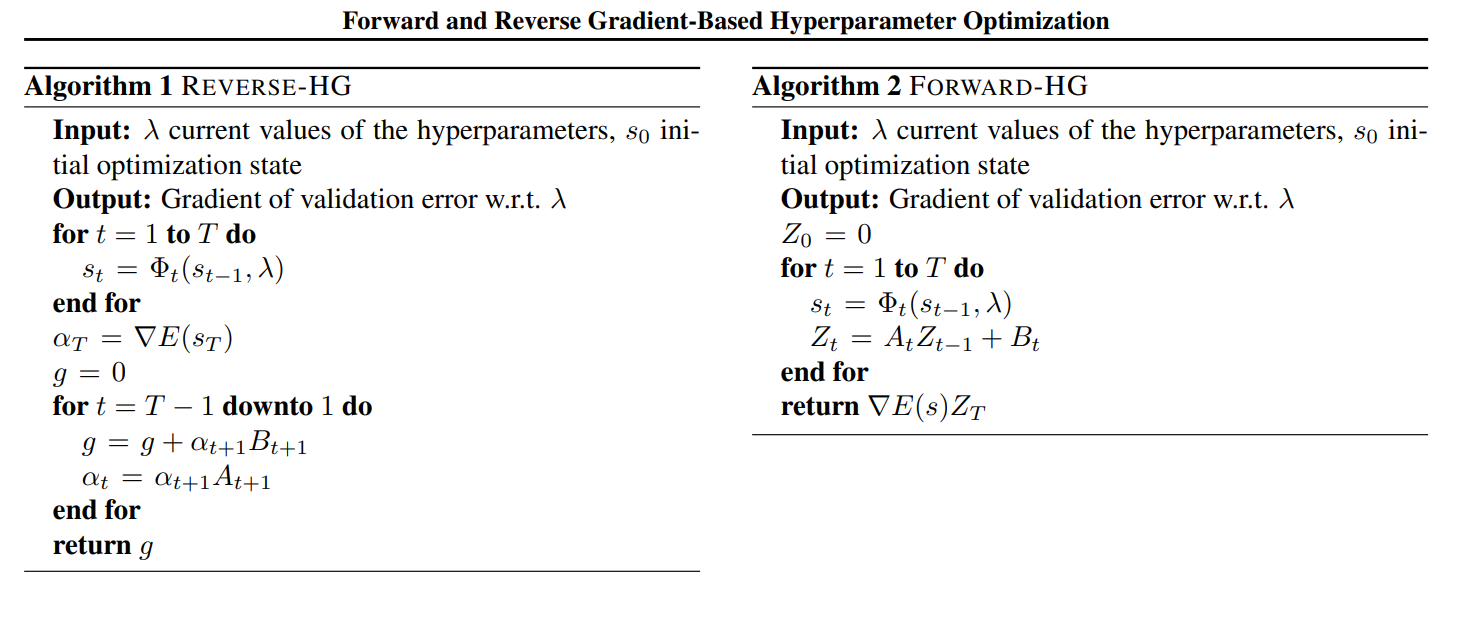
\includegraphics[scale=0.4]{images/img_algorithm.png}
    \end{figure}
\end{frame}

\section{Experiments}
\begin{frame}{Data Hyper-cleaning (MNIST)}
    \begin{figure}
        \centering
        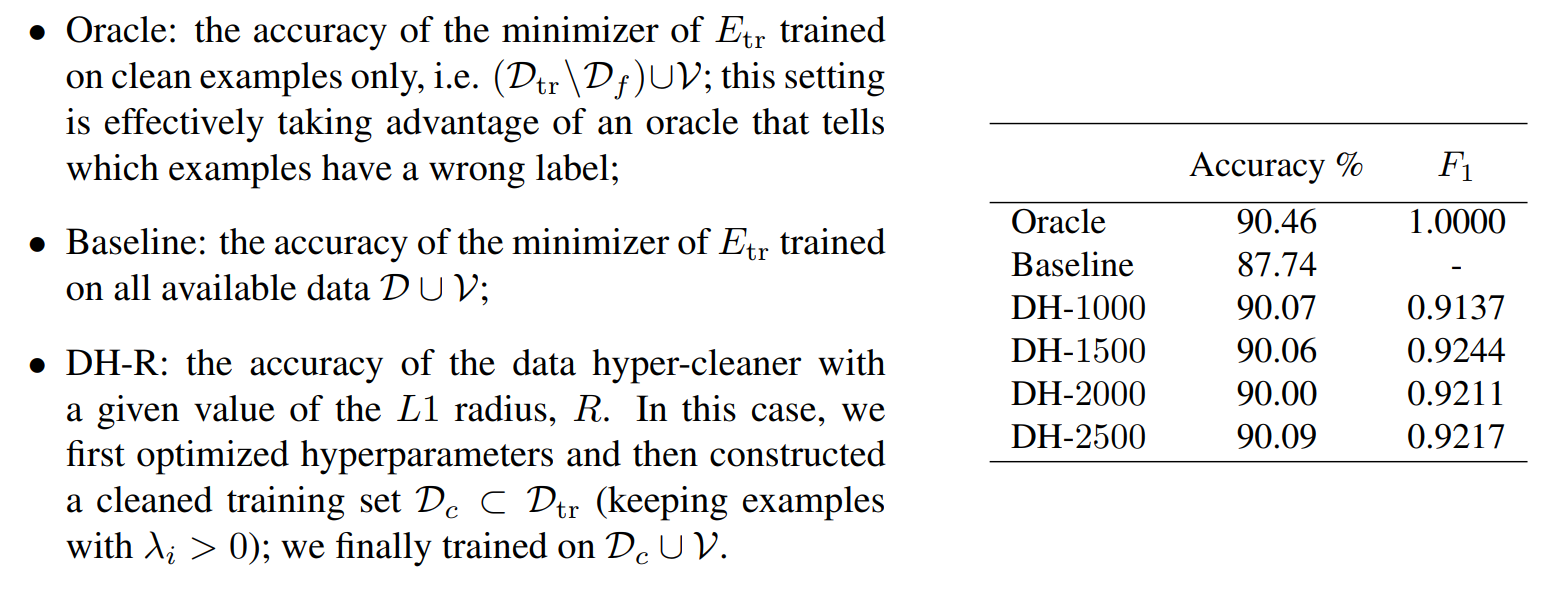
\includegraphics[scale=0.35]{images/example_1.png}
    \end{figure}
\end{frame}

\begin{frame}{Phone Classification (TIMIT)}
    \begin{figure}
        \centering
        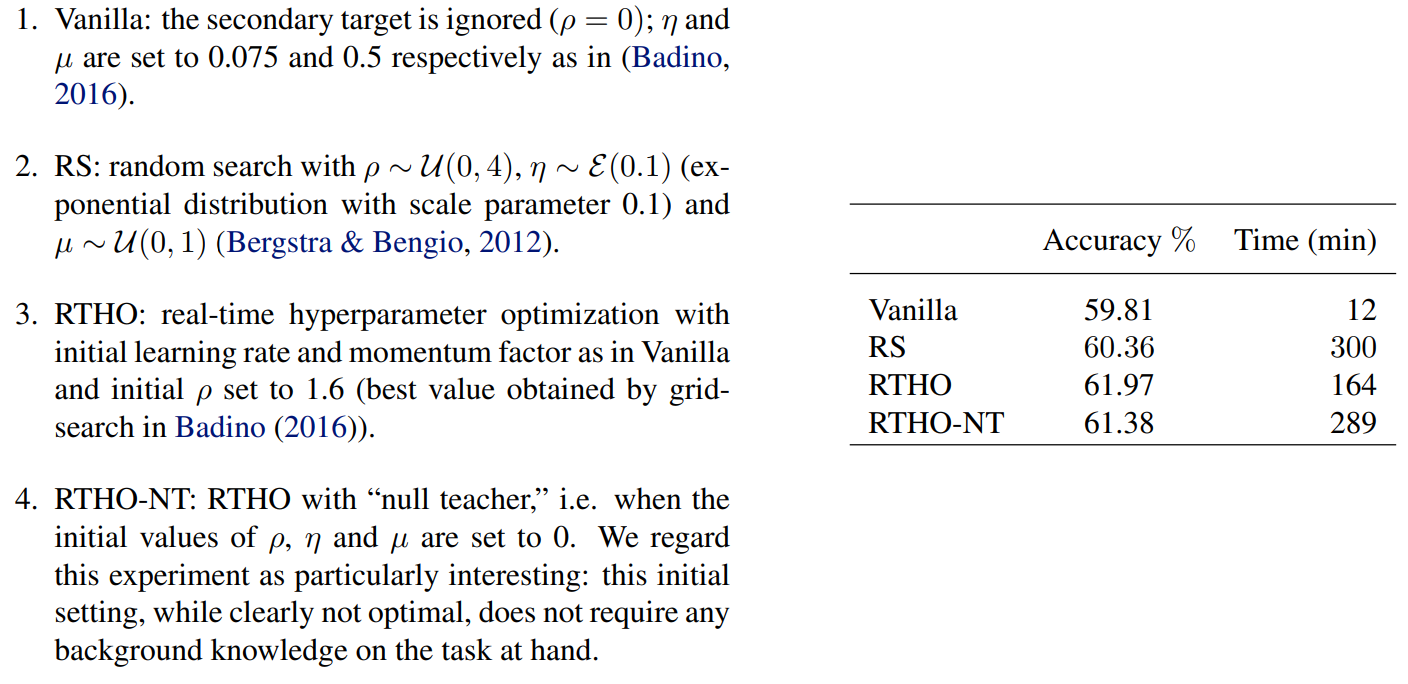
\includegraphics[scale=0.4]{images/example_2.png}
    \end{figure}
\end{frame}

\section{Literature}
\begin{frame}{Literature}
    \begin{enumerate}
        \item \textbf{Main article} \href{https://arxiv.org/pdf/1703.01785.pdf}
        {Forward and Reverse Gradient-Based Hyperparameter Optimization}.
    \end{enumerate}
\end{frame}

\end{document}